% TODO: scan for abbrs like PP, MC, SSS-MC
\chapter{Quicksand}
\label{chap:quicksand}
\inspirationalquote{
% original - on second thought, i'm not actually gonna put this in
% the nuance in japanese is more desperate, more disorganized, and less generally heroic-seeming
% i think the english translation actually works better for an inspirational quote
%{\footnotesize 嫌な事も悲しい事もあったけど、守りたい物だってたくさんこの世界にはあったから。} \\
There are awful, sad things in this world.
But there are a lot of things worth protecting, too.
}
%{Kaname Madoka, Mahou Shoujo Madoka{\raisebox{0.1em}{$\scriptstyle \bigstar$}}Magica}
% TODO: make the star italic
% TODO: see https://tex.stackexchange.com/questions/63179/shear-transform-a-box/63188#63188
{Kaname Madoka, Puella Magi Madoka{\raisebox{0.1em}{$\scriptstyle \bigstar$}}Magica}
%\inspirationalquote{Always, somewhere, someone is fighting for you.
%As long as you remember her, you are not alone.}
%{Mahou Shoujo Madoka{\raisebox{0.1em}{$\scriptstyle \bigstar$}}Magica}

% TODO: intro

% TODO: mention that all source files in this chapter are relative to id/ subdir in the repo

The contributions of this chapter were published as
{\em Stateless Model Checking with Data-Race Preemption Points}
in OOPSLA 2016 \cite{quicksand}.

%%%%%%%%%%%%%%%%%%%%%%%%%%%%%%%%%%%%%%%%%%%%%%%%%%%%%%%%%%%%%%%%%%%%%%%%%%%%%%%%
%%%%%%%%%%%%%%%%%%%%%%%%%%%%%%%%%%%%%%%%%%%%%%%%%%%%%%%%%%%%%%%%%%%%%%%%%%%%%%%%
%%%%%%%%%%%%%%%%%%%%%%%%%%%%%%%%%%%%%%%%%%%%%%%%%%%%%%%%%%%%%%%%%%%%%%%%%%%%%%%%

\section{Preemption points}
\label{sec:quicksand-pps}

% reference figure (nb color scheme tree)
% its pps were drawn on every instruction
% for larger test cases, this is not practical
% consider the example program of so and so (show mx/yield prog)
% here is a resulting state space
% this needs a DR PP to FAB
% qs example (take from thesis slides)

% TODO make sure to define maximal and mminnimal

% TODO: define "data race" (pure hb) vs "data race candidate" (limited); also do scane of this chapater for conisstencey

In related work,
Portend \cite{portend} has already suggested combining data race analysis with preemption-driven artificial scheduling,
although it obtains its data-race candidates from a stand-alone, single-pass analysis.
In order to make sure we identify every one of a program's data races that could possibly arise under the given test case,
we must check many different interleavings to begin with,
perform the Portend approach for every data race we find,
which may in turn uncover more data races
(hidden in flow control paths reachable only through interleavings of the first race, perhaps),
and then continue model checking the multiple data races together
in a sort of bidirectional feedback loop between the two algorithms.
I will refer to data races that require model checking to expose to begin with as
{\em nondeterministic data races}. % TODO: rename, this name is awful
In the next section,
\cref{sec:quicksand-id} will show how I achieve this in Quicksand, and
\cref{sec:quicksand-soundness} will justify the technique's formal verification power.
In the evaluation (\cref{sec:quicksand-eval}),
\cref{sec:quicksand-eval-nondets} in particular will justify the need
for this feedback loop between model checking and data race analysis
by showing that many bugs require nondeterministic data races to expose.

%%%%%%%%%%%%%%%%%%%%%%%%%%%%%%%%%%%%%%%%%%%%%%%%%%%%%%%%%%%%%%%%%%%%%%%%%%%%%%%%
%%%%%%%%%%%%%%%%%%%%%%%%%%%%%%%%%%%%%%%%%%%%%%%%%%%%%%%%%%%%%%%%%%%%%%%%%%%%%%%%
%%%%%%%%%%%%%%%%%%%%%%%%%%%%%%%%%%%%%%%%%%%%%%%%%%%%%%%%%%%%%%%%%%%%%%%%%%%%%%%%

\section{Iterative Deepening}
\label{sec:quicksand-id}

To address the problem of choosing meaningful preemption points,
I have developed an algorithm called {\em Iterative Deepening},
implemented in a wrapper program specific to Landslide called {\em Quicksand}.
Named after the analogous technique in chess artificial intelligence \cite{iterative-deepening-chess-ai},
Iterative Deepening
is a search strategy,
for exponentially-sized state spaces in general,
which
makes progressively deeper searches of the state space until the CPU budget is exhausted.
In this context, the depth roughly corresponds to the subset of preemption points used.
Hence, Quicksand
schedules multiple Landslide instances in parallel to
test many different subsets of the available preemption points,

For the remainder of the chapter, I will use Iterative Deepening to refer to the algorithm in the abstract,
which could in principle apply to any stateless model checking domain,
and Quicksand to refer to the specific implementation,
which relies on data race analysis and specific heuristics to optimize its testing approach
for kernels and thread libraries.
I will also henceforth refer to each unique set of preemption points as a {\em job}.

%\subsection{Design}

% TODO: put fig:id here, explain generally multiple state spaces

Note that Iterative Deepening is a {\em wrapper} algorithm around stateless MC.
A model checker is still used to test each state space, and other reduction techniques such as DPOR
are still applicable in each.
Moreover, because Iterative Deepening treats the set of preemption points as mutable,
it can add new preemption points reactively based on any runtime analysis.
Here
will focus on run-time data race analysis~\cite{tsan,fasttrack} as the mechanism for finding new preemption candidates.
The next section (\cref{sec:quicksand-soundness})
will prove that in fact,
in addition to statically-known synchronization preemption points,
this suffices to provide at least as strong verification guarantees as any other possible preemption point set.

%%%%%%%%%%%%%%%%%%%%%%%%%%%%%%%%%%%%%%%%%%%%%%%%%%%%%%%%%%%%%%%%%%%%%%%%%%%%%%%%

\subsection{Changing state spaces}

To introduce the Iterative Deepening algorithm,
I will first show a simple approach for handling new PPs in the absence of any CPU budget restriction.

Given unlimited CPU time for testing,
one would always want to switch to the new maximal state space whenever adding a new preemption point.
The maximal state space is guaranteed to subsume all execution sequences reachable in any subset state space,
so considering any incomplete subset of the known PPs would be duplicate work.
\Cref{alg:algorithm0} demonstrates this na\"ive approach.
It is seeded with the set of all statically-known synchronization API PPs,
and invoked whenever a new data-race candidate is found.
%
The upcoming proofs in \cref{sec:quicksand-soundness},
being concerned with the verification guarantee provided when the search may complete within the CPU budget,
are based on this simple version of Iterative Deepening.
The user may also wish to configure her testing tool to prefer this approach, at her discretion,
such as when she believes all bugs have been fixed and wants a verification as fast as possible;
% TODO: clarify sec reference to -M flag
\cref{sec:quicksand-implementation} discusses this execution mode further.

\newcommand\AllPPs{\ensuremath{\mathcal{A}}}
\newcommand\PendingJobs{\ensuremath{\mathcal{P}}}
\newcommand\SuspendedJobs{\ensuremath{\mathcal{S}}}
\newcommand\GetETA[1]{ETA(#1)}
\newcommand\GetPPSet[1]{PPSet(#1)}

\begin{algorithm}[h]
	\SetKwInOut{Input}{Input}
	\Input{$j$, the currently-running job}
	\Input{\AllPPs, the set of all known preemption points} %, sorted by decreasing heuristic priority}
	\eIf{$\exists p \in \AllPPs . p \not\in \GetPPSet{j}$}{
		return NewJob(\AllPPs) // New maximal state space
	}{
		return $j$ // $j$ is still maximal
	}
	\caption{Na\"ive Iterative Deepening method}
	\label{alg:algorithm0}
\end{algorithm}

However, in many tests of even modestly-sized programs,
full verification is not feasible,
and focusing on the maximal state space alone is likely to be fruitless.
%
Hence, Iterative Deepening also allows for prioritizing subset jobs
based on number of preemption points, ETA, and whether data race candidates are included among their preemption points.
It relies on state-space estimation \cite{estimation}
to predict which jobs are likely to complete within a reasonable time,
before actually testing a large fraction of interleavings for each.
The overall goal is to decide automatically when to defer testing a state space,
so an inexpert user can provide only her total CPU budget as a test parameter,
and to enable completing appropriately-sized jobs within that budget.
Quicksand seeks to maximize completed state spaces,
as each one serves as a guarantee that all interleavings possible with its PPs were tested;
\cref{sec:quicksand-discussion} discusses some limitations of this approach.
The next three subsections will show how to schedule these smaller jobs
based on their preemption points and ETAs.

%%%%%%%%%%%%%%%%%%%%%%%%%%%%%%%%%%%%%%%%%%%%%%%%%%%%%%%%%%%%%%%%%%%%%%%%%%%%%%%%

\subsection{Initial preemption points}

Iterative Deepening must be seeded with a set of initial state spaces,
which can be any number of subsets of the statically-available preemption points
that prior work model checkers would use.
The upcoming soundness proof relies on the maximal state space being included among these for verification's sake,
but to optimize for finding bugs faster,
implementations may wish to simultaneously to try testing subsets thereof.

For testing user-space code, Quicksand begins with the four jobs from \Cref{fig:id}:
$\{yield\}$,
$\{yield,lock\}$,
$\{yield,unlock\}$,
and $\{yield,lock,unlock\}$,
By extension, these also induce preemptions on any other primitives
which use
internal locks,
such as condition variables or semaphores.
Preempting on voluntary switches such as {\tt yield} is always necessary to maintain
Landslide's invariant that only one thread runs between consecutive preemption points,
so the {\tt yield} preemption point is always implicitly enabled.

For kernel-level testing, interrupt-disabling is analogous to locking,
so preemptions must also be introduced
just before a disable-interrupt opcode (on x86, {\tt cli})
and just after interrupts are re-enabled (on x86, {\tt sti}).
During data-race detection, {\tt cli} and {\tt sti} are treated as a single global lock
(note that {\tt cli}'d memory accesses can still race with others that have interrupts on).%
\footnote{Some kernels disable preemption without disabling interrupts,
which can be communicated to the MC using manual annotations,
and must be treated similarly.
This also assumes uni-processor scheduling; for SMP kernels, replace {\tt cli}/{\tt sti} with spinlocks.}
Quicksand is configured to begin with
$\{yield\}$,
$\{yield,lock\}$,
$\{yield,unlock\}$,
$\{yield,cli\}$,
$\{yield,sti\}$,
and $\{yield,lock,$ $unlock,cli,sti\}$.
As a heuristic, it doesn't test every intermediate subset such as $\{lock,sti\}$,
which would result in $2^p$ jobs right off the bat,
although this could potentially be improved in future work (\cref{sec:quicksand-discussion}).

%%%%%%%%%%%%%%%%%%%%%%%%%%%%%%%%%%%%%%%%%%%%%%%%%%%%%%%%%%%%%%%%%%%%%%%%%%%%%%%%

\subsection{Data-race preemption points}

As discussed in \cref{sec:quicksand-pps},
%runtime data race detection (\cref{sec:background-datarace})
%may find candidate unsynchronized memory conflicts that should be investigated further.
data races may beget new interleavings not reachable by preempting on synchronization API boundaries alone.
Because each data race indicates an access pair that can interleave at instruction granularity,
different program behaviour may arise if the threads are preempted just before the racing instructions,
some of which the programmer may not have even expected, i.e., be bugs,
and it is logical to apply model checking to find or verify the absence of such bugs.
%it is logical to re-execute the test and issue preemptions just before those instructions
%to test alternate thread interleavings.

With Iterative Deepening,
this is a simple matter of creating a new state space
with an additional preemption point enabled on the racing instructions by each thread,
as shown in \Cref{alg:handledatarace}.
I will term these {\em data-race preemption points},
and they will form the foundation of Quicksand's contribution.
Note that even though a data race may involve two different instructions,
$\alpha$ and $\beta$, Quicksand's strategy is to add new state spaces with only one new racing instruction at a time.
Rather than adding a single large state space,
configured to preempt on both involved instructions,
i.e., $AB =$ \GetPPSet{$j_0$} $\cup$ $\alpha$ $\cup$ $\beta$,
it prefers to add multiple smaller jobs which have a higher chance of completing in time, i.e.,
$A =$ \GetPPSet{$j_0$} $\cup$ $\alpha$ and
$B =$ \GetPPSet{$j_0$} $\cup$ $\beta$.
If $A$ and $B$ are bug-free, they will in turn add $AB$ later during their own execution.
The condition on line~1 ensures that we avoid duplicating any state spaces with multiple data-race preemption points;
for example, $AB$ is reachable by multiple paths through its different subsets $A$ and $B$,
but should of course be tested only once.

\newcommand\AllJobs{\ensuremath{\mathcal{J}}}
\begin{algorithm}[t]
	\SetKwInOut{Input}{Input}
	\Input{$j_0$, the currently-running job}
	\Input{\AllJobs, the set of all existing (or completed) jobs}
	\Input{$\alpha$, an instruction reported by the MC as part of a racing access pair}
	\If{$\forall j \in \AllJobs,$
	\GetPPSet{$j_0$} $\cup$ $\alpha$
	$\not\subseteq$
	\GetPPSet{$j$}
	}{
		AddNewJob(\GetPPSet{$j_0$} $\cup$ $\alpha$, HeuristicPriority($\alpha$)) \\
	}
	\If{$\forall j \in \AllJobs,$ \GetPPSet{$j$} $\neq \{yield, \alpha\}$}{
		AddNewJob($\{yield, \alpha\}$, HeuristicPriority($\alpha$))
	}
	\caption{Adding new jobs with data-race PPs.}
	\label{alg:handledatarace}
\end{algorithm}

Furthermore,
Iterative Deepening allows not always strictly increasing the number of preemption points
whenever a new data race is identified.
For each instruction involved in a data race, Quicksand adds two new jobs:
a ``small'' job to preempt on that instruction only (line~5),
and a ``big'' job to preempt on that instruction as well as each preemption point used by the reporting job (line~2).
%
Hence,
each {\em pair} of racing accesses will spawn four new jobs.
\Cref{fig:new-dr-jobs} visualizes the resulting overall workflow in Quicksand,
including the four such jobs resulting from one data race report.%
\footnote{As an optimization,
though the big jobs should be expected to uncover more data races and in turn
produce even bigger jobs still,
small jobs should be forbidden from ``reproducing'',
as their purpose is only fast heuristic bug-finding rather than exhaustive coverage;
see {\tt handle\_data\_race()} in {\tt messaging.c}.}
%
The rationale of spawning multiple jobs is that one cannot know in advance which will be most fruitful:
while the big job risks not completing in time,
the small job risks missing the data race entirely if the original PPs were required to expose it.
In practice, I have observed many bugs found quickly by these small jobs,
and many other bugs missed by the small jobs found eventually by the big jobs.
This phenomenon motivates Iterative Deepening to prioritize jobs at run-time.

\begin{figure}[t]
        %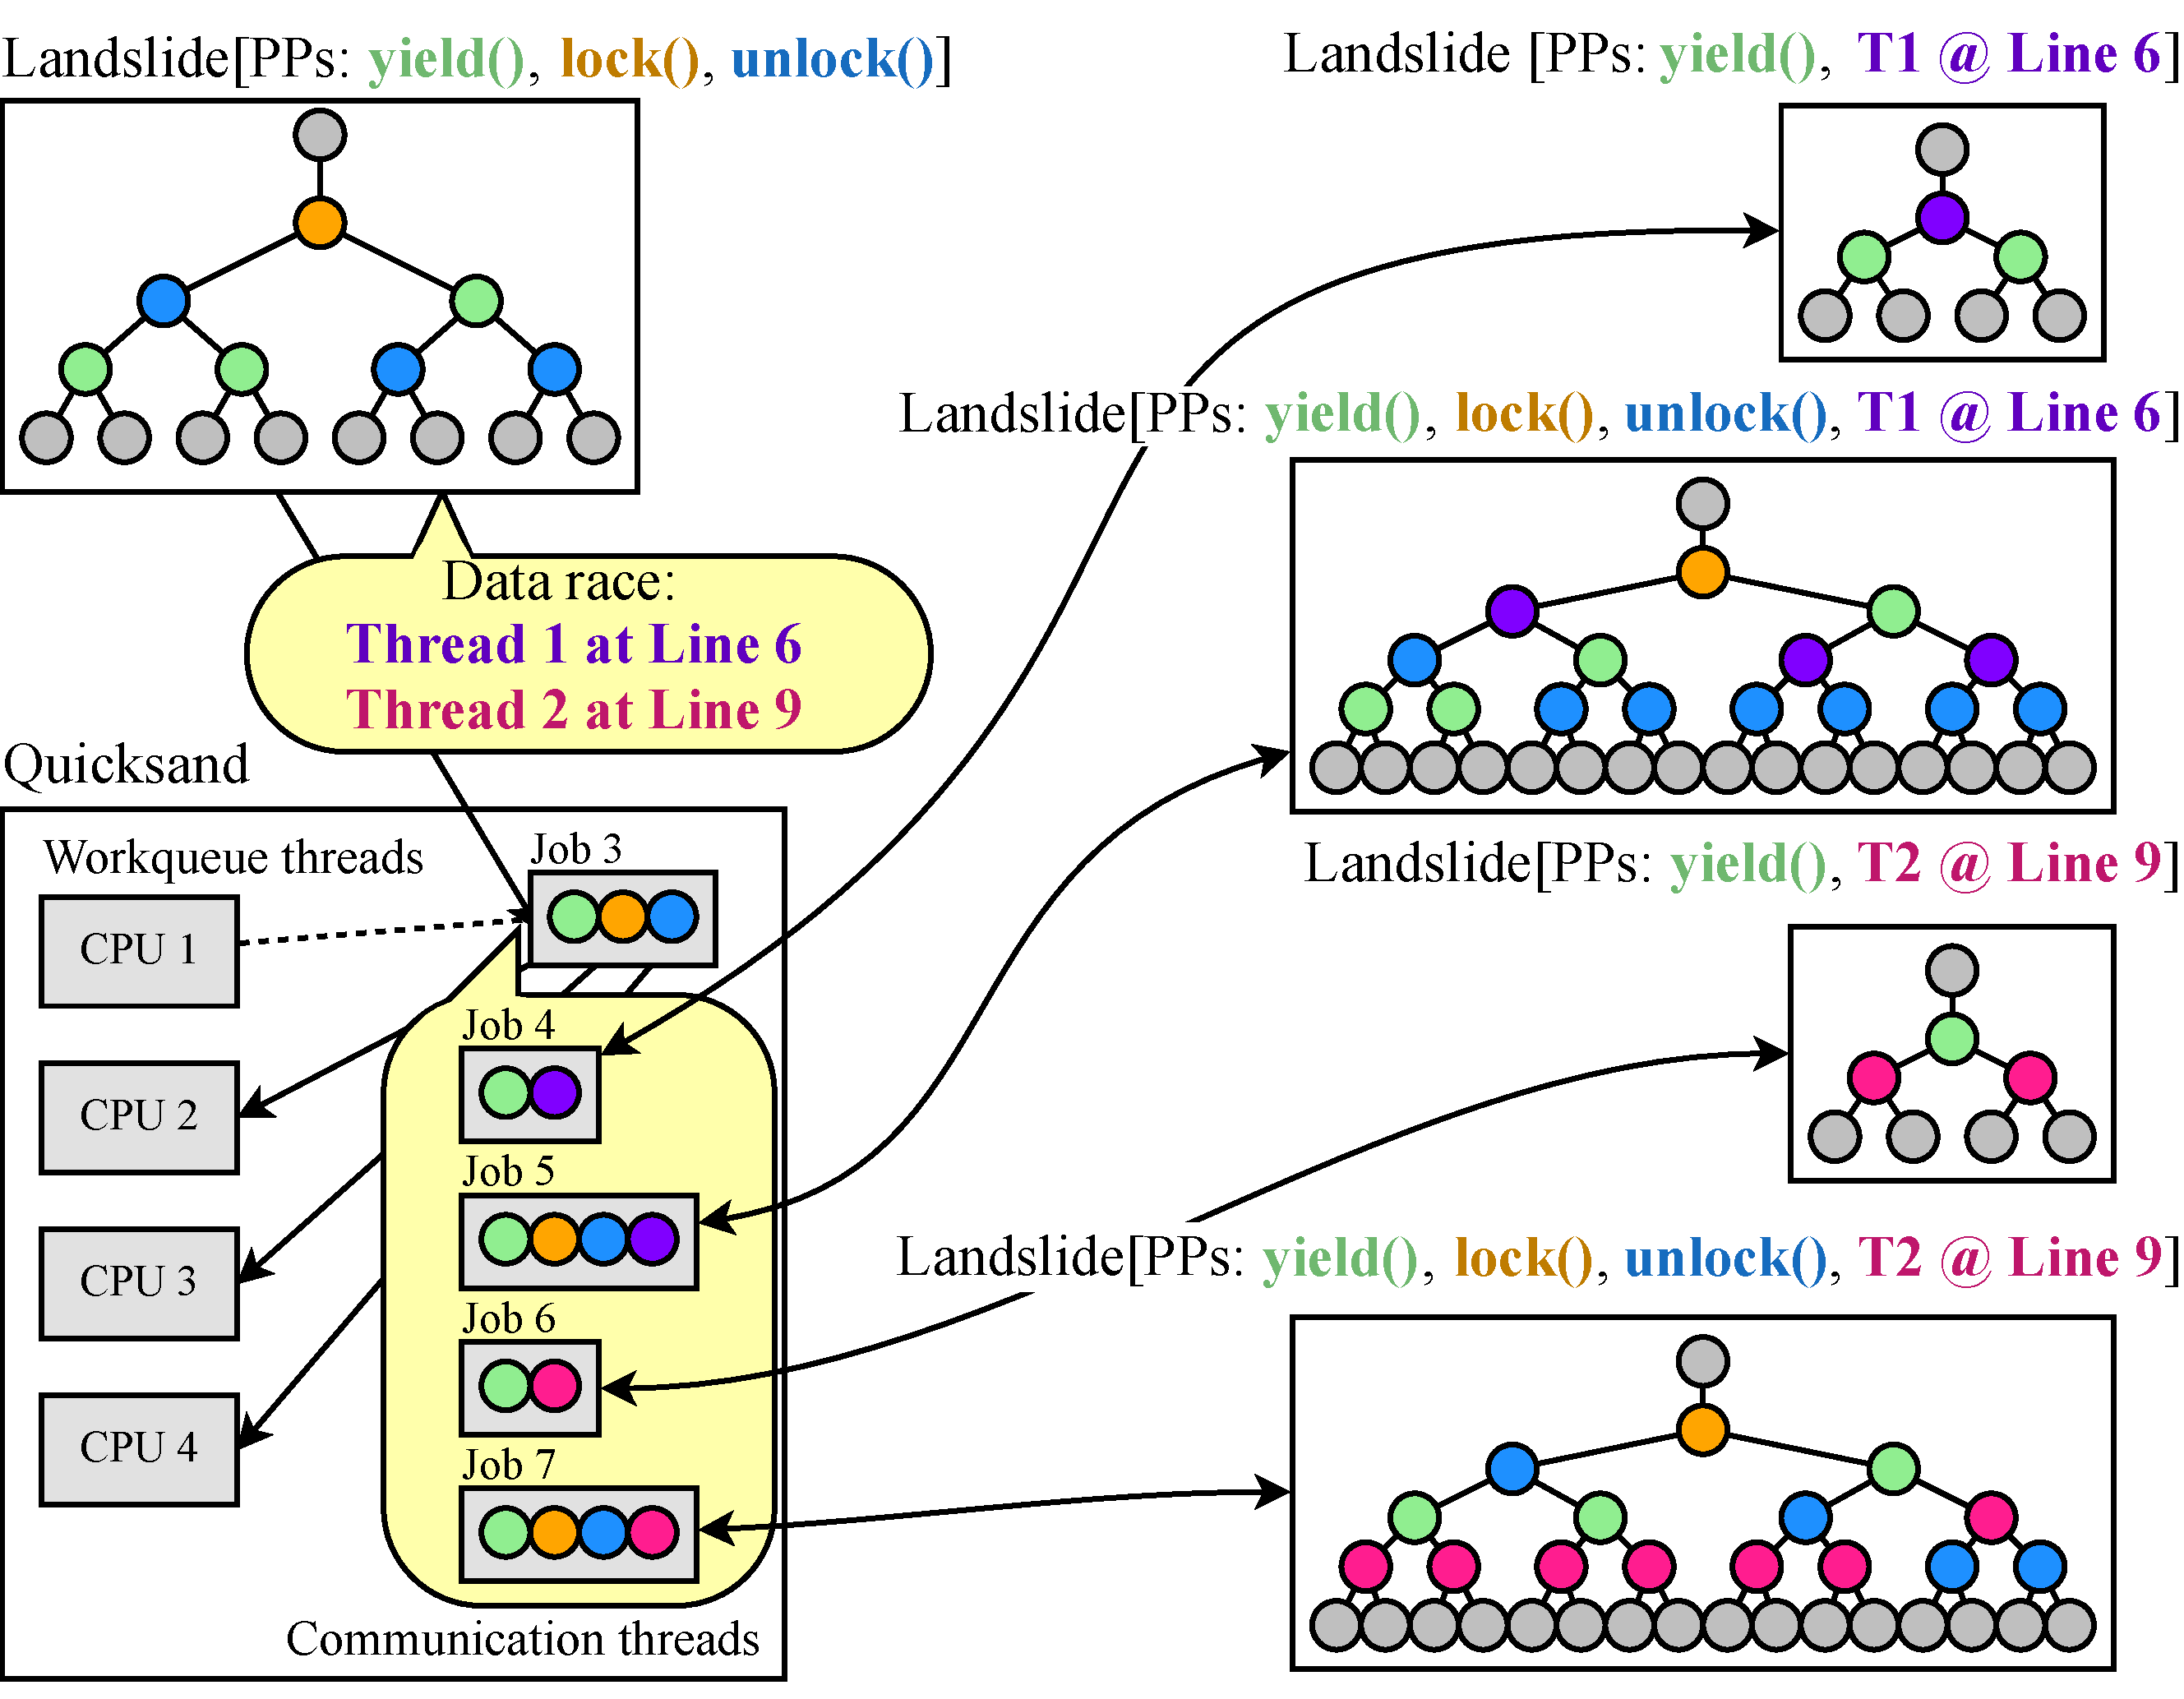
\includegraphics[width=0.48\textwidth]{dr-jobs-v2.pdf}
        asdfsaf
        % TODO: put the figure form yr snake fight
	\caption[Quicksand incorporates data race reports as new preemption points at run-time.]
		{Quicksand incorporates data race reports as new preemption points at run-time,
		by managing the exploration of multiple state spaces,
		communicating with each MC instance to receive ETAs, data race candidates, and bug reports.
                %When an access pair is reported as a data race candidate,
                When a data race is reported,
                a new preemption point is added for each involved access,
                and new jobs are added for later testing,
                corresponding to different combinations of those with the existing preemption points.}
        \label{fig:new-dr-jobs}
\end{figure}

The new state spaces may expose a failure, in which case Iterative Deepening must stop and report a data-race bug,
or complete successfully, indicating a {\em benign} (i.e., false-positive) data race.
They may also uncover a new data-race candidate entirely in some alternate interleaving,
in which case we may iteratively advance to a superset state space which will preempt at both racing access pairs.
Being constrained by a CPU budget,
Iterative Deepening may time out before completing a data race's associated state space,
in which case the data race remains neither confirmed nor refuted.
%Depending on how much burden the implementation wants to impose on the user,
%it may then report it as a
%report a potential false positive that the user must handle
In such cases, Quicksand elects to impose some burden on the user
by reporting it as a potential false positive
and recommend that she investigate it by hand to judge for herself whether it be a bug.
% TODO: fix this to point to partial verif
% TODO (also) make sure that all other quicksand-discussion references get updated if appropriate
\cref{sec:quicksand-discussion} will discuss future opportunities for improving
debugging output in cases of such {\em partial verification}.
However, experience shows that this interactivity pays off:
in the next chapter's educational user study (\cref{sec:education-eval}),
one student reported during the survey that they used this recommendation,
combined with their own intuition,
to find a bug that Quicksand was not able to find alone (\cref{sec:education-reasons-worthwhile}).

%%%%%%%%%%%%%%%%%%%%%%%%%%%%%%%%%%%%%%%%%%%%%%%%%%%%%%%%%%%%%%%%%%%%%%%%%%%%%%%%

\subsection{Choosing the best job}

With a limited CPU budget, many larger tests are likely to be fail to complete in time,
and smaller tests are likely to be more fruitful at finding bugs quickly.
A model checker's state space estimation (\cref{sec:landslide-estimate})
can provide a hint to select between these jobs.
How to handle jobs whose ETAs are too high for the given CPU budget
is the heart of Iterative Deepening,
and is listed formally in \Cref{alg:shouldworkblock}.%
\footnote{
Though its worst-case performance is $O(mn)$ in the
%number of pending and suspended jobs,
sizes of $\mathcal{P}$ and $\mathcal{S}$,
in practice the non-constant portion beyond line~4 runs very infrequently
and is negligible compared to the exponentially-sized state spaces.}.

\begin{algorithm}[t]
	\SetKwInOut{Input}{Input}
	%\textbf{Function} GetBestJob($j_0$, PendingJobs, SuspendedJobs): \\
	\Input{$j_0$, the currently-running job}
	\Input{\PendingJobs, the list of pending jobs, sorted by decreasing heuristic priority}
	\Input{\SuspendedJobs, the list of already-suspended jobs, sorted by increasing ETA}
	\Input{$T$, the remaining time in the CPU budget}
	\If{\GetETA{$j_0$} $<$ HeuristicETAFactor $\times$ $T$}{
		return $j_0$ // Common case: job is expected to finish.
	}
	\ForEach{job $j_P \in$ \PendingJobs}{
		// Don't run a pending job if a subset of it is already suspended; its ETA would be at least as bad. \\
		\If {$\forall j_S \in$ \SuspendedJobs, \GetPPSet{$j_S$} $\not\subset$ \GetPPSet{$j_P$}}{
			return $j_P$
		}
	}
	%// no pending jobs; maybe resume a suspended job \\
	\ForEach{job $j_S \in$ \SuspendedJobs}{
		\If{\GetPPSet{$j_0$} $\not\subset$ \GetPPSet{$j_S$}
			$\land$
			\GetETA{$j_0$} $>$ \GetETA{$j_S$}}{
			// If a subset of $j_S$ is also suspended, don't run the larger one first. \\
			\If{$\forall j_{S2} \in$ \SuspendedJobs, \GetPPSet{$j_{S2}$} $\not\subset$ \GetPPSet{$j_S$}}{
				return $j_S$
			}
		}
	}
	return $j_0$ // \GetETA{$j_0$} was bad, but no other $j$ was better.
	\caption{Suspending exploration of a state space in favor of a potentially smaller one.}
	\label{alg:shouldworkblock}
\end{algorithm}

Its main feature is understanding that if \GetPPSet{$j_1$} $\subset$ \GetPPSet{$j_2$},
and $j_1$ is suspended,
then $j_2$'s state space is guaranteed to be strictly larger, so $j_2$ will take at least as long.
Hence, as long as $j_1$ is suspended on account of being too big,
$j_2$ should not be tested either,
unless $j_1$ is later resumed and its ETA improves over time after further execution.
%reveals that it might finish in time after all.
Similarly, whenever a job finds a bug, all pending superset jobs may safely be cancelled,
as they are guaranteed to contain the same program behaviour, and likely to simply find the same bug again.
%
Implementation-wise,
Quicksand receives an updated estimate from each Landslide instance whenever it finishes executing a new interleaving,
and separates them accordingly
into a set of {\em suspended} jobs,
i.e., partially-explored state spaces with high ETAs,
and a set of {\em pending} jobs,
i.e., untested ones with unknown ETAs.
When Landslide reports an ETA too high for some job,
it is compared with other pending and suspended jobs to find another one more likely to complete in time.%
\footnote{Note that when Quicksand is configured to use multiple CPUs,
simultaneously-running jobs are not considered among the set of possible jbos to switch to,
so if there are fewer total jobs with ETA lower than the time budget than the allowed parallelism factor,
some CPUs may end up speculatively running large jobs
in hopes that the ETA turns out to be an overestimate.}

Iterative Deepening also accounts for the inherent inaccuracy of ETA estimates.
Line~1 heuristically scales up the time remaining to avoid suspending jobs too aggressively
in case their ETAs are actually overestimated.
Lines~12-15 account for the
%bizarre
possibility that among two suspended jobs,
%given two jobs,
%%$j_1,j_2$,
\GetPPSet{$j_1$} $\subset$ \GetPPSet{$j_2$}
but
\GetETA{$j_1$} $>$ \GetETA{$j_2$}.
This may seem surprising,
but can often arise because estimates tend to get more accurate over time,
and $j_1$ perhaps ran much longer, on account of being overall smaller,
before becoming suspended.
In such scenarios,
the algorithm heuristically assumes the smaller job's ETA is more accurate,
in order to avoid repeatedly resuming larger jobs briefly only to find that their ETAs keep getting worse and worse
(in other words, it lets us avoid thrashing in Quicksand). % ¯\_(ツ)_/¯

%%%%%%%%%%%%%%%%%%%%%%%%%%%%%%%%%%%%%%%%%%%%%%%%%%%%%%%%%%%%%%%%%%%%%%%%%%%%%%%%

\subsection{Heuristics}

As predicting the ETAs of state spaces of unknown size
and using that plus size of a set of preemption points as a proxy for how likely a job is to find bugs or complete
is a fundamentally messy process,
it is appropriate to equip the algorithm with some heuristics informed by experience.
\Cref{alg:shouldworkblock} allows the option to heuristically scale a job's ETA
when comparing it to the overall time budget,
which can compensate for any inaccuracy by the estimator.
Quicksand uses a scaling factor defaulting to 2,
chosen based on experiments from prior work \cite{estimation}.
%though we allow changing it via the command line.
It also includes a heuristic to
never suspend jobs before they pass a certain threshold of interleavings tested,
with a default of 32,
informed by my personal experience that ETAs require around that much progress into the state space
before they stabilize (at least relative to each other on similar state spaces,
not necessarily relative to the ultimate true size).%
\footnote{These two heuristics are configurable with the
{\tt -e} and {\tt -E} command-line options, respectively,
as discussed in \cref{sec:landslide-quicksand-options}.}

Landslide classifies data-race candidates as {\em both-order} or {\em single-order},
as defined in prior work \cite{portend},
based on whether it observed the racing instructions ordered in both possible sequences or only one
in the original state space, respectively.
Single-order candidates are more likely to be false positives (\cref{sec:background-datarace}),
although preempting during the access itself is necessary to say for sure.
Hence, Quicskand add preemption points for both types of candidates,
and heuristically prioritizes jobs with both-order data races
over those with only single-order data races.
The HeuristicPriority($\alpha$) call in \Cref{alg:handledatarace} corresponds to this strategy.
For single-order races, Quicksand does not initially add a PP for the later access at all:
if preempting on the first access is capable of reordering the race,
it will be updated to both-order in the new state space, and the second preemption point will be added then.
\cref{sec:warpzone-heuristics} will discuss opportunities for future work to expand
these heuristics with more nuanced search strategies still.

%%%%%%%%%%%%%%%%%%%%%%%%%%%%%%%%%%%%%%%%%%%%%%%%%%%%%%%%%%%%%%%%%%%%%%%%%%%%%%%%

\subsection{Reallocation false positives}
\label{sec:quicksand-id-realloc}

Finally, I identified a particular class of false positive data-race candidates
under the Limited Happens-Before analysis (\cref{sec:background-datarace})
in which the associated memory was recycled by re-allocation between the two accesses,
and claim that it is safe to completely disregard them when considering where to add new preemption points.
Figure~\ref{fig:recycle} shows a common code pattern and interleaving which can expose such behaviour.
If the {\tt malloc} on line~4 returns the same address passed to {\tt free} on line~2,
then lines~1 and 7 will be flagged as a potential data race.
I term this a {\em reallocation false-positive data-race candidiate}.
To the human eye, this is obviously a false positive:
reordering lines~4-7 before lines~1-2 will cause {\tt malloc} to return a different region of allocated memory,
in turn causing {\tt x} and {\tt y} to no longer collide.
In studying a similar pattern, the Eraser tool from prior work \cite{eraser}
found that Thread 2's logic usually corresponds to an initialization pattern,
but for generality I have added an arbitrary {\tt publish} action to the example on line~6.

% TODO: fix syntax hilight
% TODO check figure placement
% TODO check figure camption
\begin{figure}[t]
	\begin{center}
	\begin{tabular}{rll}
		& \multicolumn{2}{c}{\texttt{struct x \{ int foo; int baz; \} *x;}} \\
		& \multicolumn{2}{c}{\texttt{struct y \{ int bar; \} *y;~~~~~~~~~~}} \\
		\\
		& {\bf Thread 1} & {\bf Thread 2} \\
		1 & \texttt{\hilight{brickred}{x->foo = ...;}} & \\
		2 & \texttt{\hilight{olivegreen}{free}(x);} \\
		3 & & \texttt{\hilight{commentblue}{// x's memory reallocated}} \\
		4 & & \texttt{y~=~\hilight{olivegreen}{malloc}(sizeof *y);} \\
		5 & & \texttt{\hilight{commentblue}{// ...initialize...}}\\
		6 & & \texttt{publish(y);} \\
		7 & & \texttt{\hilight{brickred}{y->bar = ...;}} \\
	\end{tabular}
	\end{center}
	\caption{A common execution pattern with {\tt malloc()} that produces false positive data race candidates.}
	\label{fig:recycle}
\end{figure}

As long as the allocation heap is properly synchronized,
a Pure Happens-Before analysis should identify a happens-before edge
between line~2's {\tt free} and line~4's {\tt malloc},
and it would report no race.
However, the upcoming evaluation will show that Limited Happens-Before retains some advantages over Pure
(\cref{sec:quicksand-eval-bugs}),
so it is useful to be able to automatically suppress data-race candidates
that are certain to end up being false positives when reordered.

The ability to disregard reallocation false positives is unique to Iterative Deepening.
When limited to a single test execution, suppressing any data race candidate matching this pattern is unsound.
Consider the more unusual program in Figure~\ref{fig:recycle-bug},
in which the memory is recycled the same way, but the racing access's address is not tied to {\tt malloc}'s return value.
Here, reordering lines~6-7 before line~3 will allow {\tt x} and {\tt x2} to race.
Such collisions could instead be avoided with a hacked allocator which never recycles memory,
but this could unacceptably impact performance in {\tt malloc}-heavy tests.
Moreover,
in the context of Iterative Deepening, being able to discard certain data race candidates
allows Quicksand to skip exploring some entire state spaces,
and hence run fewer Landslides overall;
this is analogous to DPOR's ability to skip equivalent interleavings within a single Landslide instance.
Upcoming in the evaluation, \cref{sec:quicksand-eval-verif}'s \Cref{tab:drstatistics}
will show how many redundant state spaces Quicksand is able to prune with this technique.

% TODO smae as above
\begin{figure}[t]
	\begin{tabular}{rll}
		& {\bf Thread 1} & {\bf Thread 2} \\
		1 & \texttt{publish(x);} & \\
		2 & \texttt{\hilight{brickred}{x->foo = ...;}} & \\
		3 & \texttt{\hilight{olivegreen}{free}(x);} \\
		4 & & \texttt{x2 = get\_published\_x();} \\
		5 & & \texttt{\hilight{commentblue}{// x's memory recycled}} \\
		6 & & \texttt{y~=~\hilight{olivegreen}{malloc}(sizeof *y);} \\
		7 & & \texttt{\hilight{brickred}{x2->foo = ...;}} \\
	\end{tabular}
	\caption{If a single-pass \revision{Limited HB analysis}~discarded candidates matching the malloc-recycle pattern,
it would miss the bug in this adversarial program.}
	\label{fig:recycle-bug}
\end{figure}

%%%%%%%%%%%%%%%%%%%%%%%%%%%%%%%%%%%%%%%%%%%%%%%%%%%%%%%%%%%%%%%%%%%%%%%%%%%%%%%%

\section{Soundness}
\label{sec:quicksand-soundness}

Adding new data-race preemption points in a feedback loop can uncover bugs
not previously reachable by preempting on synchronization APIs alone,
as some prior model checkers do \cite{dbug-ssv},
but how does it compare to the other extreme end of the trade-off,
that is,
committing in advance to preempt on every single shared memory access \cite{inspect}?
It turns out,
assuming sufficient CPU budget,
Iterative Deepening can in principle expose every possible program behaviour that
even that latter approach can find,
providing an equally strong verification guarantee.
This section presents a proof of this claim (\cref{sec:quicksand-convergence}),
as well as a supplementary proof (\cref{sec:quicksand-realloc})
of the soundness of pruning reallocation false positives discussed previously (\cref{sec:quicksand-id-realloc}).

I am presenting these proofs as they appeared in the OOPSLA paper \cite{quicksand}:
written as sketches in informal prose,
to optimize for rapidly conveying an intuition for why it works
rather than to justify every internal step within the proof structure.%
\footnote{Also because I am already over 200 pages in this thesis, all told.}
% footnote yeah, i'm writing this last
% footnote of footnote yeah, the committee never read this part
A more rigorous treatment
is available in the tech report which accompanied the conference paper \cite{quicksand-soundness}.

{\bf Assumptions.}
The proofs are built on a DPOR definition which assumes sequentially-consistent memory hardware.
All algorithms involved are assumed to operate on a machine model of a single globally-consistent execution trace,
which fundamentally cannot account for memory reordering nondeterminism.
\cref{sec:quicksand-discussion} discusses this limitation further;
for existing work on combining DPOR with relaxed memory, I refer the reader to \cite{tsopso}.
They also assume the Limited Happens-Before definition
for the data-race analysis.
I leave the case for Pure Happens-Before to future work,
although if I may appeal to intuition,
it requires only to show that for any data-race candidate
Limited Happens-Before reports in a given execution,
that Pure Happens-Before does not,
either it will be a false positive,
or the latter will find it in an alternate execution within the same state space,
or the latter will find a different data race that ultimately leads to a bigger state space in which the first one may be found.

\subsection{Convergence}
\label{sec:quicksand-convergence}

\subsubsection{Equivalence}

% TODO: decide if this shouldn't be reordered befor econvergence?
\subsubsection{Saturation}

\subsection{Reallocation false positives}
\label{sec:quicksand-realloc}

% todo rename "malloc recycle" to "reallocation false positives"

%%%%%%%%%%%%%%%%%%%%%%%%%%%%%%%%%%%%%%%%%%%%%%%%%%%%%%%%%%%%%%%%%%%%%%%%%%%%%%%%
%%%%%%%%%%%%%%%%%%%%%%%%%%%%%%%%%%%%%%%%%%%%%%%%%%%%%%%%%%%%%%%%%%%%%%%%%%%%%%%%
%%%%%%%%%%%%%%%%%%%%%%%%%%%%%%%%%%%%%%%%%%%%%%%%%%%%%%%%%%%%%%%%%%%%%%%%%%%%%%%%

\section{Implementation}
\label{sec:quicksand-implementation}

% TODO: add -M flag discussion

% TODO: cant swap x100

% TODO: put a code snippet of what ap rogress report looks like (take from some htm log)

% this section developers guide to quicksand

% job
% messaging
% work
% option
% pp

% cool tricks
% cant swap x100 % cite [Inf09] ?

% how is free re malloc implemented in landslide?

%%%%%%%%%%%%%%%%%%%%%%%%%%%%%%%%%%%%%%%%%%%%%%%%%%%%%%%%%%%%%%%%%%%%%%%%%%%%%%%%
%%%%%%%%%%%%%%%%%%%%%%%%%%%%%%%%%%%%%%%%%%%%%%%%%%%%%%%%%%%%%%%%%%%%%%%%%%%%%%%%
%%%%%%%%%%%%%%%%%%%%%%%%%%%%%%%%%%%%%%%%%%%%%%%%%%%%%%%%%%%%%%%%%%%%%%%%%%%%%%%%

\section{Evaluation}
\label{sec:quicksand-eval}

\subsection{Finding bugs}
\label{sec:quicksand-eval-bugs}

\subsection{Verification}
\label{sec:quicksand-eval-verif}

\subsection{Nondeterministic data races}
\label{sec:quicksand-eval-nondets}

%%%%%%%%%%%%%%%%%%%%%%%%%%%%%%%%%%%%%%%%%%%%%%%%%%%%%%%%%%%%%%%%%%%%%%%%%%%%%%%%
%%%%%%%%%%%%%%%%%%%%%%%%%%%%%%%%%%%%%%%%%%%%%%%%%%%%%%%%%%%%%%%%%%%%%%%%%%%%%%%%
%%%%%%%%%%%%%%%%%%%%%%%%%%%%%%%%%%%%%%%%%%%%%%%%%%%%%%%%%%%%%%%%%%%%%%%%%%%%%%%%

\section{Discussion}
\label{sec:quicksand-discussion}

% identifying & skipping redundancies in smaller ID state spaces via memoization (same applies to ICB!)

%%%%%%%%%%%%%%%%%%%%%%%%%%%%%%%%%%%%%%%%%%%%%%%%%%%%%%%%%%%%%%%%%%%%%%%%%%%%%%%%
%%%%%%%%%%%%%%%%%%%%%%%%%%%%%%%%%%%%%%%%%%%%%%%%%%%%%%%%%%%%%%%%%%%%%%%%%%%%%%%%
%%%%%%%%%%%%%%%%%%%%%%%%%%%%%%%%%%%%%%%%%%%%%%%%%%%%%%%%%%%%%%%%%%%%%%%%%%%%%%%%

\section{Summary}

quicksand is gr9
